\documentclass[]{report}
\usepackage{lmodern}
\usepackage{amssymb,amsmath}
\usepackage{ifxetex,ifluatex}
\usepackage{fixltx2e} % provides \textsubscript
\ifnum 0\ifxetex 1\fi\ifluatex 1\fi=0 % if pdftex
  \usepackage[T1]{fontenc}
  \usepackage[utf8]{inputenc}
\else % if luatex or xelatex
  \ifxetex
    \usepackage{mathspec}
  \else
    \usepackage{fontspec}
  \fi
  \defaultfontfeatures{Ligatures=TeX,Scale=MatchLowercase}
\fi
% use upquote if available, for straight quotes in verbatim environments
\IfFileExists{upquote.sty}{\usepackage{upquote}}{}
% use microtype if available
\IfFileExists{microtype.sty}{%
\usepackage{microtype}
\UseMicrotypeSet[protrusion]{basicmath} % disable protrusion for tt fonts
}{}
\usepackage[margin=1in]{geometry}
\usepackage{hyperref}
\hypersetup{unicode=true,
            pdfauthor={Samuel Lippl},
            pdfborder={0 0 0},
            breaklinks=true}
\urlstyle{same}  % don't use monospace font for urls
\usepackage{natbib}
\bibliographystyle{apalike}
\usepackage{color}
\usepackage{fancyvrb}
\newcommand{\VerbBar}{|}
\newcommand{\VERB}{\Verb[commandchars=\\\{\}]}
\DefineVerbatimEnvironment{Highlighting}{Verbatim}{commandchars=\\\{\}}
% Add ',fontsize=\small' for more characters per line
\usepackage{framed}
\definecolor{shadecolor}{RGB}{248,248,248}
\newenvironment{Shaded}{\begin{snugshade}}{\end{snugshade}}
\newcommand{\AlertTok}[1]{\textcolor[rgb]{0.94,0.16,0.16}{#1}}
\newcommand{\AnnotationTok}[1]{\textcolor[rgb]{0.56,0.35,0.01}{\textbf{\textit{#1}}}}
\newcommand{\AttributeTok}[1]{\textcolor[rgb]{0.77,0.63,0.00}{#1}}
\newcommand{\BaseNTok}[1]{\textcolor[rgb]{0.00,0.00,0.81}{#1}}
\newcommand{\BuiltInTok}[1]{#1}
\newcommand{\CharTok}[1]{\textcolor[rgb]{0.31,0.60,0.02}{#1}}
\newcommand{\CommentTok}[1]{\textcolor[rgb]{0.56,0.35,0.01}{\textit{#1}}}
\newcommand{\CommentVarTok}[1]{\textcolor[rgb]{0.56,0.35,0.01}{\textbf{\textit{#1}}}}
\newcommand{\ConstantTok}[1]{\textcolor[rgb]{0.00,0.00,0.00}{#1}}
\newcommand{\ControlFlowTok}[1]{\textcolor[rgb]{0.13,0.29,0.53}{\textbf{#1}}}
\newcommand{\DataTypeTok}[1]{\textcolor[rgb]{0.13,0.29,0.53}{#1}}
\newcommand{\DecValTok}[1]{\textcolor[rgb]{0.00,0.00,0.81}{#1}}
\newcommand{\DocumentationTok}[1]{\textcolor[rgb]{0.56,0.35,0.01}{\textbf{\textit{#1}}}}
\newcommand{\ErrorTok}[1]{\textcolor[rgb]{0.64,0.00,0.00}{\textbf{#1}}}
\newcommand{\ExtensionTok}[1]{#1}
\newcommand{\FloatTok}[1]{\textcolor[rgb]{0.00,0.00,0.81}{#1}}
\newcommand{\FunctionTok}[1]{\textcolor[rgb]{0.00,0.00,0.00}{#1}}
\newcommand{\ImportTok}[1]{#1}
\newcommand{\InformationTok}[1]{\textcolor[rgb]{0.56,0.35,0.01}{\textbf{\textit{#1}}}}
\newcommand{\KeywordTok}[1]{\textcolor[rgb]{0.13,0.29,0.53}{\textbf{#1}}}
\newcommand{\NormalTok}[1]{#1}
\newcommand{\OperatorTok}[1]{\textcolor[rgb]{0.81,0.36,0.00}{\textbf{#1}}}
\newcommand{\OtherTok}[1]{\textcolor[rgb]{0.56,0.35,0.01}{#1}}
\newcommand{\PreprocessorTok}[1]{\textcolor[rgb]{0.56,0.35,0.01}{\textit{#1}}}
\newcommand{\RegionMarkerTok}[1]{#1}
\newcommand{\SpecialCharTok}[1]{\textcolor[rgb]{0.00,0.00,0.00}{#1}}
\newcommand{\SpecialStringTok}[1]{\textcolor[rgb]{0.31,0.60,0.02}{#1}}
\newcommand{\StringTok}[1]{\textcolor[rgb]{0.31,0.60,0.02}{#1}}
\newcommand{\VariableTok}[1]{\textcolor[rgb]{0.00,0.00,0.00}{#1}}
\newcommand{\VerbatimStringTok}[1]{\textcolor[rgb]{0.31,0.60,0.02}{#1}}
\newcommand{\WarningTok}[1]{\textcolor[rgb]{0.56,0.35,0.01}{\textbf{\textit{#1}}}}
\usepackage{longtable,booktabs}
\usepackage{graphicx,grffile}
\makeatletter
\def\maxwidth{\ifdim\Gin@nat@width>\linewidth\linewidth\else\Gin@nat@width\fi}
\def\maxheight{\ifdim\Gin@nat@height>\textheight\textheight\else\Gin@nat@height\fi}
\makeatother
% Scale images if necessary, so that they will not overflow the page
% margins by default, and it is still possible to overwrite the defaults
% using explicit options in \includegraphics[width, height, ...]{}
\setkeys{Gin}{width=\maxwidth,height=\maxheight,keepaspectratio}
\IfFileExists{parskip.sty}{%
\usepackage{parskip}
}{% else
\setlength{\parindent}{0pt}
\setlength{\parskip}{6pt plus 2pt minus 1pt}
}
\setlength{\emergencystretch}{3em}  % prevent overfull lines
\providecommand{\tightlist}{%
  \setlength{\itemsep}{0pt}\setlength{\parskip}{0pt}}
\setcounter{secnumdepth}{5}

%%% Use protect on footnotes to avoid problems with footnotes in titles
\let\rmarkdownfootnote\footnote%
\def\footnote{\protect\rmarkdownfootnote}

%%% Change title format to be more compact
\usepackage{titling}

% Create subtitle command for use in maketitle
\newcommand{\subtitle}[1]{
  \posttitle{
    \begin{center}\large#1\end{center}
    }
}

\setlength{\droptitle}{-2em}

  \title{}
    \pretitle{\vspace{\droptitle}}
  \posttitle{}
    \author{Samuel Lippl}
    \preauthor{\centering\large\emph}
  \postauthor{\par}
      \predate{\centering\large\emph}
  \postdate{\par}
    \date{2018-09-30}

\usepackage{booktabs, titlesec, blindtext}
\usepackage[svgnames]{xcolor}
\hypersetup{
    bookmarksnumbered=true,
    bookmarksopen=false,
    bookmarksopenlevel=1,
    colorlinks=true,
    linkcolor=blue,
    urlcolor=DarkBlue,
    citecolor=DarkRed
}
\definecolor{chgray}{gray}{0.5}
\newcommand{\hsp}{\hspace{20pt}}
\titleformat{\chapter}[hang]{\Huge\bfseries}{\thechapter\hsp\textcolor{chgray}{|}\hsp}{0pt}{\Huge\bfseries}

\usepackage{amsthm}
\newtheorem{theorem}{Theorem}[chapter]
\newtheorem{lemma}{Lemma}[chapter]
\theoremstyle{definition}
\newtheorem{definition}{Definition}[chapter]
\newtheorem{corollary}{Corollary}[chapter]
\newtheorem{proposition}{Proposition}[chapter]
\theoremstyle{definition}
\newtheorem{example}{Example}[chapter]
\theoremstyle{definition}
\newtheorem{exercise}{Exercise}[chapter]
\theoremstyle{remark}
\newtheorem*{remark}{Remark}
\newtheorem*{solution}{Solution}
\let\BeginKnitrBlock\begin \let\EndKnitrBlock\end
\begin{document}

\begin{titlepage}

% Titlepage inspired by: https://www.overleaf.com/15991102jmmvbxxtbhfk#/61015645/

\newcommand{\HRule}{\rule{\linewidth}{0.5mm}} % Defines a new command for the horizontal lines, change thickness here

\center % Center everything on the page

%----------------------------------------------------------------------------------------
%	TITLE SECTION
%----------------------------------------------------------------------------------------

\HRule \\[0.4cm]
{ \huge \bfseries Outlier Detection using Regression in R}\\[0.4cm] % Title of your document
\HRule \\[1.5cm]

%----------------------------------------------------------------------------------------
%	HEADING SECTIONS
%----------------------------------------------------------------------------------------

\textsc{\LARGE Ludwig-Maximilians-Universität München}\\[0.5cm] % Name of your university/college
\textsc{\Large Fakultät für Mathematik, Informatik und Statistik}\\[1.5cm]


\textsc{\Large Seminar "Ausreißer- und Anomaliedetektion" von Prof. Dr. Christian Heumann}\\[0.5cm] % Major heading such as course name
\textsc{\large Hausarbeit}\\[0.5cm] % Minor heading such as course title

%----------------------------------------------------------------------------------------
%	LOGO SECTION
%----------------------------------------------------------------------------------------

\vfill

\includegraphics[height=0.2\textheight]{figs/sigill.png}\\[1cm] % Include a department/university logo - this will require the graphicx package



%----------------------------------------------------------------------------------------
%	DATE SECTION
%----------------------------------------------------------------------------------------

\vfill

%----------------------------------------------------------------------------------------
%	AUTHOR SECTION
%----------------------------------------------------------------------------------------

{\Large 30. September 2018}\\[1cm]
\begin{Large}
\textsc{Autor}\\Samuel Lippl
\end{Large}

\vfill

\end{titlepage}

\pagenumbering{roman}
\setcounter{page}{2}

\chapter*{Selbständigkeitserklärung}

Ich erkläre hiermit, dass ich die vorliegende Arbeit selbständig angefertigt, alle Zitate als solche kenntlich gemacht sowie alle benutzten Quellen und Hilfsmittel angegeben habe.\\

\begin{tabular}{c}
\\\\\\
\\\hline
Samuel Lippl, 30.09.2018
\end{tabular}

\hypertarget{abstract}{%
\chapter*{Abstract}\label{abstract}}


This report will provide an overview over outlier detection in R. It
starts by discussing some general principles of outlier detection.
Linear methods and their nonlinear extensions are presented next. Along
the general methods, examples of application and an appropriate
methodology in R are introduced.

\tableofcontents

\hypertarget{intro}{%
\chapter{Introduction: neurons, models and outliers}\label{intro}}

\pagenumbering{arabic}
\setcounter{page}{1}

In the late 1990s, neuroscientists faced a curious problem. They
investigated a set of neurons which started to fire when a bar with a
certain orientation appeared within their receptive field, i. e. the
visual area these neurons were concerned with. However, when this bar
extended their receptive field, the firing stopped. This behaviour is
called \emph{endstopping}.

\begin{figure}
\includegraphics[width=1\linewidth]{outlier-detection_files/figure-latex/endstopping-1} \caption{Illustration of endstopping: The shaded rectangle
shows the receptive field of the neuron. The black rectangle represents
the bar. If the receptive field is grey, the neuron does not fire, if it
is orange, the neuron fires.}\label{fig:endstopping}
\end{figure}






Different functions of these endstopped neurons had been postulated.
Studies had suggested a role for these cells in detecting curvature,
line terminations, occlusion, perceptual grouping and illusory contours.
\citep{Rao1999} Rao and Ballard's study presented an alternative
explanation for this effect. Their analysis suggested that higher-level
neurons whose receptive field resembled the entire area in figure
\ref{fig:endstopping} predicted the lower-level input. Feedback
connections transmitted the error of the transmission. According to Rao
and Ballard, the endstopped neurons had the function of error feedback.

They demonstrated this by fitting a hierarchical model with three layers
on image patches extracted from five natural photos such that the
higher-level layers optimally predicted the lower-level layers. The
feedback nodes encoding the difference between the values in the second
layer and the values that had been predicted by the third layer
exhibited endstopping effects. \citep{Rao1999}

The explanation for neuronal endstopping therefore consists of two
parts: firstly, the structure of neuronal networks allow for association
of neighbouring pixels which is necessary to detect bars. Secondly,
short bars are less usual than longer bars\footnote{Rao and Ballard
  demonstrated this by another investigation \citep{Rao1999}.}. This is
the reason why the higher-level neurons predict a longer bar in these
cases and receive a higher error feedback signal. Short bars are
therefore \emph{outliers}. Endstopped neurons thus provide a natural
example for outlier detection.

Since these investigation, predictive coding, the hypothesis that
higher-level neuronal layers attempt to predict lower-level layers, has
become popular with respect to different areas of the brain
\citep{Friston2005}. Intuitively, this makes sense: if the received
input represents usual patterns the information of the higher-level
neurons suffices so that lower-level correction is only required if
something unusual happens. This allows the brain to build a model of
reality as such a model cannot account for all irregularities and retain
its descriptive power. Consider, for instance, a chess game where the
player attempts to predict his opponent's actions. It is impossible to
consider all possible moves. Instead, the player has to restrict himself
to the most probable ones. If the next move has been considered by the
player, his opponent behaves in the usual way and the player can rest
assured. In contrast, if the player has not considered the next move, he
may be alerted. Unusual behavior therefore merits special attention, in
particular, if it is impossible to model all paths of behavior.

The statistical implementation of this strategy is given by outlier
detection. The examples are manifold:

\begin{itemize}
\tightlist
\item
  It is impossible to model all possible methods to commit credit card
  fraud. Instead, we simply try to detect unusual behavior.
\item
  There are many different reasons why data points may deviate from the
  assumptions of the classical linear model but many of these deviations
  are observable by looking at different kinds of residual errors.
\item
  There are many different reasons why a sensor can be corrupted and not
  all of them can be considered. However, many of them manifest
  themselves in unusual patterns.
\end{itemize}

\emph{Outliers} can now be defined as those data points that are
\emph{dissimilar from the other data points}
\citep[see][]{Aggarwal2017}. The particular outlier detection methods
defines what it means for data points to be similar to each other. For
instance, with respect to the endstopping neurons, image patches are
similar if they can be characterized by the same neuronal model.

This report focuses on methods that generate predictions and assess them
in order to judge how \emph{usual} a certain data point is. Its
structure is based on chapter 3 of Aggarwal's \emph{Outlier Analysis}
\citeyearpar{Aggarwal2017}. Two alternative popular approaches are
probabilistic modeling \citep[ch.~2]{Aggarwal2017} and clustering
\citep[ch.~4]{Aggarwal2017}. Note that the distinction is not
well-defined and there are many methods that can be attributed to
different fields (see \protect\hyperlink{methods}{chapter 2}).

\protect\hyperlink{methods}{Chapter 2} presents a general methodology to
assess outlier scores and introduces the \emph{Z-plot} as a
visualization of outlier scores..

Subsequently, \protect\hyperlink{linear}{chapter 3} introduces outlier
detection using linear models and principal component analysis. All
these methods are limited by the fact that they can only model linear
relationships. This disadvantage is adressed in
\protect\hyperlink{nonlinear}{chapter 4} where nonlinear extensions of
these methods are introduced. Specifically, the kernel trick is
introduced yielding kernel principal component analysis. Finally, more
complex regressions, in particular neural networks, are introduced.
Methodological instructions consist of the following parts:

\begin{itemize}
\tightlist
\item
  \textbf{Motivation} and \textbf{intuition}: What does it mean for a
  data point to be usual? What hyperparameters need to be adjusted and
  how do they affect whether data points are usual?
\item
  \textbf{Implementation} in R
\item
  Example \textbf{application}: a two-dimensional outlier analysis using
  different generated datasets should provide an intuition for
  advantages and disadvantages of every method as it is visually easy to
  assess
\item
  Applications in \textbf{compression} and data \textbf{correction}, two
  related fields to outlier detection
\item
  \textbf{Pro} and \textbf{Contra}
\end{itemize}

\hypertarget{methodology}{%
\chapter{Methodology}\label{methodology}}

This chapter introduces the methods with which the outlier detection
algorithms are discussed in the following. It first discusses the
connection between data compression, data correction, outlier labels and
outlier scores, embeds methods using regression in alternatives using
probabilistic modeling or clustering and then presents \emph{Z-Scoring}
as a simple heuristic to normalize outlier scores. Finally, evaluation
of outlier scores, both in this report and in general are discussed and
toy outlier datasets are introduced.

\hypertarget{a-nested-account-of-outlier-detection}{%
\section{A nested account of outlier
detection}\label{a-nested-account-of-outlier-detection}}

Outlier detection is closely related to the fields of data compression
and data correction. In fact, there is a canonical connection which will
be discussed in this section. Firstly, let us produce a definition of
the different general algorithms.

\BeginKnitrBlock{definition}
\protect\hypertarget{def:unnamed-chunk-1}{}{\label{def:unnamed-chunk-1}
}Consider some data \(D\in\mathcal{D}^n,n\in\mathbb{N}\). An algorithm
\(A\) achieves

\begin{enumerate}
\def\labelenumi{\alph{enumi})}
\item
  \textbf{data compression} if and only if it yields an \emph{encoding
  procedure} \[E^D:\mathcal{D}\to\mathcal{C}\] (where \(\mathcal{C}\) is
  some compressed space) and a \emph{decoding procedure}
  \[F^D:\mathcal{C}\to\mathcal{D}.\] Consider, for instance, a large
  file \(D\in\mathcal{D}\) where \(\mathcal{D}\) is the space of files
  of a certain maximum size. The zipping algorithm DEFLATE uses --
  broadly speaking -- repeating \textbf{pattern}s in the files to reduce
  size by relating repeated \textbf{pattern}s to the original
  \textbf{pattern}. For instance, the highlighted string sequence
  ``pattern'' in the last sentence occurred thrice -- the latter two
  times, it could have been replaced by a reference to the original
  sequence. DEFLATE would thus produce a compressed (zipped) file
  \(Z=E^D(D)\) which can then be decoded to yield the original data file
  \(D = F^D(Z)\). \citep[see][]{Group1996}

  This is an example of \emph{lossless} data compression. In many cases,
  however, data is compressed in such a way that it cannot be entirely
  recovered. This is called \emph{lossy} data compression. I will
  illustrate the procedure by a simple example. Suppose that the data
  consists of a set of geometrical figures. We detect that they are all
  rectangles and we can therefore save them by the width and height.
  This data compression is lossless. If we wish to compress the data
  even further, we might note that most rectangles are approximately
  squares and we can encode them by the mean of their width and height.
  If, for instance a rectangle of width 5.0 cm and height 6.0 cm is
  encoded, we save the number 5.5 (encoded). In the decoding step, we
  convert the number 5.5 into a square of width and height 5.5 cm.
  Whereas this is not exactly the rectangle we put in, we may decide
  that it is close enough.
\item
  \textbf{data correction} if and only if it yields a \emph{correction
  procedure} \[C^D:\mathcal{D}^n\to\mathcal{D}^n\] such that \(C^D(D)\)
  is a corrected version of \(D\). In our working example, data
  correction would imply a different perspective on our
  rectangle-square-problem. Perhaps, we know that all geometrical forms
  are supposed to be squares but there has been some measurement error.
  The product could then be viewed as a computation of the most likely
  square that has been measured in the first place. Generally, we do not
  need a framework with encoding and decoding -- another solution would
  be, for example, to assume the lesser value of width and height as the
  actual value of both width and height.
\item
  \textbf{outlier scoring} if and only if it can label each data point
  \(d\in\mathcal{D}\) with a score that captures the dissimilarity of
  \(d\) compared to the dataset \(D\). This would, again, imply a
  different perspective: perhaps, not all measured forms have been
  squares but they have usually been approximate squares. Then, the
  rectangles with large differences between width and height are unusual
  observations and some measure like the absolute difference between
  width and height captures the degree to which they are outliers --
  their \emph{outlier score}. Of course, we could also try to measure
  how different the corrected form (the square) is from the original
  form (the rectangle). The larger the difference, the larger the
  outlier score.
\item
  \textbf{outlier labels} if and only if it can label each data point
  \(d\in\mathcal{D}\) with a binary label that indicates whether it is
  an outlier score or not. For instance, we might define, that those
  rectangles are outliers where width and height have a difference of
  more than 1 cm.
\end{enumerate}
\EndKnitrBlock{definition}

Outlier scoring and labeling are a part of outlier detection and we will
discuss their relation in the next section. At this point, I will work
out the implied relations between the different algorithms, namely:

\begin{itemize}
\tightlist
\item
  A \emph{data compression} algorithm can be used for \emph{data
  correction} by viewing the encoded and then decoded data as corrected
  data.
\item
  A \emph{data correction} algorithm can be used for \emph{outlier
  scoring} by measuring the dissimilarity between the original and the
  corrected data.
\item
  An \emph{outlier scoring} algorithm can be used for \emph{outlier
  labels} by defining a threshold such that any data point with a larger
  outlier score is defined as an outlier.
\end{itemize}

This implies a nested account of outlier detection and allows us to
further our understanding of capable outlier detection algorithms by
regarding them as compressing and correcting algorithms. More
explicitly, an unusual observation is one that cannot be compressed as
much without a large margin of error, resp. one that differs a lot from
its corrected version. Both perspectives therefore contribute to our
understanding of outlier detection algorithms and I will regard them
where appropriate.

It remains to remark that, of course, data compression algorithms are
not, per se, superior to pure outlier detection algorithms just because
they also induce a method of the latter category. If the latter
algorithm has a better performance in detecting outliers in a certain
situation, it is evidently better at this task, even if it is not
capable of data compression.

\hypertarget{context-probabilistic-and-cluster-analysis-for-outlier-detection}{%
\section{Context: Probabilistic and cluster analysis for outlier
detection}\label{context-probabilistic-and-cluster-analysis-for-outlier-detection}}

While this report introduces regression methods for outlier detection,
this is not the only option. In its most basic form, outlier detection
consists of a collection of real numbers \(x_1,\dotsc, x_n\) and the
suspicious data points are ``too'' far at the borders of the dataset.
This is the domain of \emph{extreme value analysis}. A useful outlier
score in this context is the standardized deviation from the mean (often
referred to as the \emph{Z-Score}):
\[z_i=|x_i-\hat{\mu}|/\hat{\sigma}, \hat{\mu}=\frac{\sum_{j=1}^nx_j}{n}, \hat{\sigma}=\sqrt{\frac{\sum_{j=1}^n(x_j-\hat{\mu})^2}{n}}\]
Theoretically, this is motivated by a normal distribution as, in this
case, a higher value of \(z_i\) implies a lower probability of \(x_i\).
However, as long as the anomalies lie at the borders of the data, the
score provides a good heuristic even under non-normal assumptions. As a
general rule of thumb, Aggarwal suggests that data points with Z scores
\(z_i>=3\) are to be treated as outliers. \citep[p.~6]{Aggarwal2017}

Probabilistic outlier detection can also handle more complex data, the
elementary assumption being that unusual data is improbable data
\citep[for a general introduction, see][ch.~2]{Aggarwal2017}. An
important application is the multivariate analog of the univariate
Z-score: if \(\mu\in\mathbb{R}^d\) is the (estimated or actual) mean and
\(\Sigma\in\mathbb{R}^{d\times d}\) is the (estimated or actual)
covariance matrix, we define the \emph{Mahalanobis score} for an
observation \(x\in\mathbb{R}^d\) by

\[M(x,\mu,\Sigma):=\sqrt{(x-\mu)^T\Sigma^{-1}(x-\mu)}\]

If the data follows a multivariate normal distribution, a higher score,
again, implies a lower probability. The Mahalanobis score also accounts
for correlations within the data -- other methods like the
\emph{Expectation Maximization algorithm} are able to capture
arbitrarily complex patterns in the data \citep{Dempster1977}.

What use do regression methods have, then? I would argue that there is a
two-fold shift. Firstly, regression methods do not always model
probabilities. As seen in the next chapter, there are certain
circumstances in which its probabilities are not the most important
determinant of whether a data point is an outlier. Secondly, the focus
on the relation between the different dimensions of the data yields a
higher explanatory power of the outlier detection score. In contrast,
probabilistic methods are rendered inflexible by certain assumptions,
namely a data point is an outlier if it has low probability.

Analogously, \emph{clustering outlier detection} focus on the connection
between observations instead of dimensions. They determine usual regions
within the dataset, i. e. \emph{clusters}. A data point is an outlier if
it does not belong to any cluster. A general introduction can be found
in Aggarwal \citeyearpar[ch.~4]{Aggarwal2017}.

Finally, there is an important application of extreme value analysis
within regression outlier detection. Many of these methods yield outlier
scores. However, these scores are scaled differently and it is therefore
not immediately clear what values correspond to outliers. However, only
data points with particularly high scores can be outliers -- the scores
therefore adhere to the assumptions of extreme value analysis. The next
section will present a general heuristic that uses Z-scoring to
normalize outlier scores.

\hypertarget{z-scoring-a-heuristic-for-normalization-of-outlier-scores}{%
\section{Z-Scoring: A heuristic for normalization of outlier
scores}\label{z-scoring-a-heuristic-for-normalization-of-outlier-scores}}

Oftentimes, outlier detection algorithms yields scores which capture
some kind of absolute deviation from the expected value -- the value is
nonnegative and a larger value implies that the data point conforms less
the patterns in the data. However, the orders of magnitude may be very
different: a value of 1 might imply a strict outlier in one case whereas
a value of 100 might be well within the expected deviations in another
case. I present a heuristic that presupposes that any outlier score
\(o_i\) of a data point \(i\) can be written as

\[
o_i=|\tilde{x}_i-\tilde{\mu}|
\]

where \(\tilde{\mu}\) is the expected value of \(\tilde{x}_i\). Clearly,
this corresponds to the intuition of outlier scores that the larger
value implies a stronger possibility that \(i\) is indeed an outlier. We
can now standardize this through the means of \emph{extreme value
analysis}: the latent variable \(\tilde{\mu}\) does not even have to be
estimated. On the other hand, \(\sigma\), the standard deviation of
\(\tilde{x}_i\) may be estimated by

\[
\hat{\sigma}=
\frac{1}{n}\sum_{i=1}^n(\tilde{x}_i-\tilde{\mu})^2=
\frac{1}{n}\sum_{i=1}^n|\tilde{x}_i-\tilde{\mu}|^2=
\frac{1}{n}\sum_{i=1}^no_i^2,
\]

which implies that we do not need the latent variable \(\tilde{\mu}\)
for the estimation. Note that we have normalized by \(n\) and not
\(n-1\) as we do not lose a degree of freedom because we do not estimate
the mean \(\tilde{\mu}\).

Under our presuppositions, we have therefore now determined a value
which broadly conforms to standardized rules of thumb: more specifically
we will look at the thresholds \(2\) (narrow), \(3\) (recommended by
Aggarwal) and \(4\) (rather high). The aforementioned \emph{Z-plot}
visualizes this standardization in a consistent way by using the
following palette from the package \texttt{scico} \citep{scico}:

\begin{Shaded}
\begin{Highlighting}[]
\NormalTok{out_pal <-}\StringTok{ "lajolla"}
\end{Highlighting}
\end{Shaded}

Furthermore, we will cap the values at \(4\) by assuming that every
value above this threshold can safely be considered an outlier. This is
ensured by the following transformation:

\begin{Shaded}
\begin{Highlighting}[]
\NormalTok{out_breaks <-}\StringTok{ }\KeywordTok{c}\NormalTok{(}\DecValTok{0}\NormalTok{, }\DecValTok{1}\NormalTok{, }\DecValTok{2}\NormalTok{, }\DecValTok{3}\NormalTok{, }\DecValTok{4}\NormalTok{)}
\NormalTok{out_trans <-}\StringTok{ }\KeywordTok{trans_new}\NormalTok{(}\StringTok{"out"}\NormalTok{, }\DataTypeTok{transform =} \ControlFlowTok{function}\NormalTok{(x) }\KeywordTok{pmax}\NormalTok{(}\KeywordTok{pmin}\NormalTok{(x, }\DecValTok{4}\NormalTok{), }\DecValTok{0}\NormalTok{),}
                       \DataTypeTok{inverse =} \ControlFlowTok{function}\NormalTok{(x) x,}
                       \DataTypeTok{breaks =} \ControlFlowTok{function}\NormalTok{(limits) }\DecValTok{0}\OperatorTok{:}\DecValTok{4}\NormalTok{,}
                       \DataTypeTok{minor_breaks =} \ControlFlowTok{function}\NormalTok{(limits) }\KeywordTok{seq}\NormalTok{(}\DecValTok{0}\NormalTok{, }\DecValTok{4}\NormalTok{, }\FloatTok{.5}\NormalTok{))}
\end{Highlighting}
\end{Shaded}

We therefore define the following visualization as a Z-plot:

\begin{Shaded}
\begin{Highlighting}[]
\NormalTok{err_marg <-}\StringTok{ }\FloatTok{.05}
\NormalTok{zplot <-}\StringTok{ }\ControlFlowTok{function}\NormalTok{(df, x, y, outlier, }\DataTypeTok{errmarg =}\NormalTok{ err_marg, }\DataTypeTok{show.legend =} \OtherTok{FALSE}\NormalTok{) \{}
  \KeywordTok{ggplot}\NormalTok{(df, }\KeywordTok{aes_string}\NormalTok{(}\DataTypeTok{x =}\NormalTok{ x, }\DataTypeTok{y =}\NormalTok{ y, }\DataTypeTok{fill =}\NormalTok{ outlier)) }\OperatorTok{+}
\StringTok{    }\KeywordTok{geom_tile}\NormalTok{(}\DataTypeTok{show.legend =}\NormalTok{ show.legend) }\OperatorTok{+}
\StringTok{    }\KeywordTok{scale_fill_scico}\NormalTok{(}\DataTypeTok{palette =}\NormalTok{ out_pal, }\DataTypeTok{trans =}\NormalTok{ out_trans, }\DataTypeTok{limits =} \KeywordTok{c}\NormalTok{(}\DecValTok{0}\NormalTok{, }\DecValTok{4}\NormalTok{),}
                     \DataTypeTok{labels =}
                       \ControlFlowTok{function}\NormalTok{(breaks) }\KeywordTok{paste}\NormalTok{(breaks, }\StringTok{"s"}\NormalTok{)) }\OperatorTok{+}
\StringTok{    }\NormalTok{my_theme }\OperatorTok{+}
\StringTok{    }\KeywordTok{theme}\NormalTok{(}\DataTypeTok{legend.position =} \StringTok{"top"}\NormalTok{) }\OperatorTok{+}
\StringTok{    }\KeywordTok{geom_tile}\NormalTok{(}\DataTypeTok{data =}\NormalTok{ df[}\KeywordTok{abs}\NormalTok{(df[[outlier]] }\OperatorTok{-}\StringTok{ }\DecValTok{3}\NormalTok{) }\OperatorTok{<=}\StringTok{ }\NormalTok{errmarg, ],}
              \DataTypeTok{fill =} \StringTok{"black"}\NormalTok{) }\OperatorTok{+}
\StringTok{    }\KeywordTok{geom_tile}\NormalTok{(}\DataTypeTok{data =}\NormalTok{ df[}\KeywordTok{abs}\NormalTok{(df[[outlier]] }\OperatorTok{-}\StringTok{ }\DecValTok{2}\NormalTok{) }\OperatorTok{<=}\StringTok{ }\NormalTok{errmarg }\OperatorTok{|}
\StringTok{                                     }\KeywordTok{abs}\NormalTok{(df[[outlier]] }\OperatorTok{-}\StringTok{ }\DecValTok{4}\NormalTok{) }\OperatorTok{<=}\StringTok{ }\NormalTok{errmarg, ],}
              \DataTypeTok{fill =} \StringTok{"gray"}\NormalTok{)}
\NormalTok{\}}
\end{Highlighting}
\end{Shaded}

Let us look at the simple example in figure \ref{fig:norm-ex}.

\begin{figure}

{\centering \includegraphics[width=0.5\linewidth]{outlier-detection_files/figure-latex/norm-ex-1} 

}

\caption{Example for a Z-plot: the \(L_2\)-norm}\label{fig:norm-ex}
\end{figure}



Any value above \(4\) is now simply black which allows the plot to be
compared across outlier detection algorithms as the colourbar remains
constant. Furthermore, the inner gray circle refers to a threshold of
\(2\) whereas the outer gray circle refers to a threshold of \(4\). The
black circle in the middle corresponds to the value \(3\). These are
intended to visualize the outlier areas according to these three
thresholds more clearly. Together, the Z-plot provides a good first look
into the results of a certain outlier detection algorithm in two
dimensions. We will therefore now discuss two-dimensional example data.

\hypertarget{evaluation-of-outlier-detection-algorithms}{%
\section{Evaluation of outlier detection
algorithms}\label{evaluation-of-outlier-detection-algorithms}}

The discussion of anomaly benchmark datasets by \citet{Emmott2015} has a
few implications for the evaluation of algorithms in this report:
firstly, they point out that artificial data is almost always too simple
and therefore not fit for a fair evaluation of outlier detection
algorithms. They therefore advocate constructing benchmark data for this
evaluation by modifying real datasets. In terms of characterizing these
datasets, they identify four problem dimensions of anomaly detection:

\begin{itemize}
\tightlist
\item
  \emph{point difficulty}: how different are the outliers from the
  normal data points?
\item
  \emph{semantic variation}: how different are the processes which
  create the different outliers? If many outliers are generated by the
  same process, this patterns might be captured by the algorithm which
  would yield unfavorable results.
\item
  \emph{relative frequency}: how many data points are anomalies of
  interest?
\item
  \emph{feature relevance}: how many of the feature dimensions are
  relevant/irrelevant for the task at hand?
\end{itemize}

The scope of this report is too narrow to include a detailed evaluation
of the different algorithms. Instead, I will refer to other evaluations
talk about influences of these four dimensions where they are evident.
As a small visualization of the algorithms, I will introduce four
datasets with different difficulties and outlier patterns. These can be
seen in figure \ref{fig:ex-data}.

\begin{figure}
\includegraphics[width=1\linewidth]{outlier-detection_files/figure-latex/ex-data-1} \caption{Example datasets}\label{fig:ex-data}
\end{figure}

In the following chapters, I will distinguish outliers and normal data
points by shape.

Clearly, these datasets represent different levels of difficulty --
regarding the sinusoidal pattern, there might not even be accordance on
the outliers between humans. Furthermore, I do not claim that these
datasets represent a fair evaluation of the algorithms. They are only
intended as simple examples of application. I will therefore not report
the detection accuracy as this would implicitly rank the algorithms
without a proper methodology. I also point out that the linear, circular
and quadratic patterns are very difficult in terms of their little
semantic variation.

\hypertarget{linear}{%
\chapter{Linear Outlier Detection}\label{linear}}

Regression starts with a linear model -- many nonlinear methods are
essentially extensions of linear methods. It is therefore sensible to
begin this exposition with the linear methods, as well. We will first
discuss linear models and then go on to discuss principal component
analysis.

\hypertarget{linear-model}{%
\section{Linear Models}\label{linear-model}}

Linear Models are the most common regression technique and therefore a
fitting start for a discussion of outlier detection algorithms using
regression.

\hypertarget{motivation}{%
\subsection{Motivation}\label{motivation}}

Consider a few examples: suppose we compare the performance of students
a lecture with their grades after the exam. Alternatively, we compare
the level of education with the pay grade or the forecast with the
actual weather. In all these cases, our intuition for outliers is rather
clear: how strongly does the latter dimension deviate from the
prediction of the former? These are \textbf{instances} of a directed
model which may be implemented by a linear model. We therefore extract a
certain feature which should conform to the prediction by the other
feature. A larger deviation would imply a stronger possibility that a
certain data point is an outlier.

\hypertarget{definition-and-implementation-in-r}{%
\subsection{Definition and implementation in
R}\label{definition-and-implementation-in-r}}

\BeginKnitrBlock{definition}
\protect\hypertarget{def:unnamed-chunk-5}{}{\label{def:unnamed-chunk-5}
}Consider data points \(i\in\{1,\dotsc,n\}\) with covariates
\(X\in\mathbb{R}^{n\times p}\) and a predicted variable
\(Y\in\mathbb{R}^n\). \emph{Outlier detection with a linear model} first
estimates the least squares fit of the linear model and then predicts
all data points from their covariates. The deviation \(|\hat{y}_i-y_i|\)
is the resulting outlier score.
\EndKnitrBlock{definition}

The implementation is simple:

\begin{enumerate}
\def\labelenumi{\arabic{enumi}.}
\item
  Fit a linear model with the function \texttt{lm}.
\item
  Predict the data points and determine the residuals with
  \texttt{predict}.
\end{enumerate}

\hypertarget{example-application}{%
\subsection{Example application}\label{example-application}}

\begin{figure}
\centering
\includegraphics{outlier-detection_files/figure-latex/lin-ex-1.pdf}
\caption{\label{fig:lin-ex}Outlier detection using linear models}
\end{figure}

The application of this method to the example data can be found in
figure \ref{fig:lin-ex}. The linear pattern is recognized rather well
which is partly due to the evenly distributed outliers. The algorithm
fails to recognize the correct patterns in the nonlinear cases for
obvious reasons.

\hypertarget{data-compression-and-correction}{%
\subsection{Data compression and
correction}\label{data-compression-and-correction}}

Data compression would be achieved by leaving out the predicted variable
and decoding the compressed pattern by predicting it according to the
fitted linear model. Data correction would correspond to replacing the
true value of the predicted variable by its prediction from the other
variables.

\hypertarget{discussion}{%
\subsection{Discussion}\label{discussion}}

It is important to emphasize at this point that such a simple model will
scarcely be useful for many different reasons. From a practical point of
view, the dynamics in most real-world datasets cannot be captured by a
linear assumption. This restriction applies to all methods in this
chapter. However, this method can easily be extended to arbitrary
regressions which are able to capture more complex relationships. This
enables us to extract features, prevent overfitting and adress other
issues with the help of regression methods. On the other hand, special
knowledge is necessary to apply a directed model -- after all, we need
to know which variable to predict. In the aforementioned examples, this
has worked -- in particular, these methods may often be applied in a
spatiotemporal context \citep[ch.~9 and 11]{Aggarwal2017} in which we
predict data at time point \(t\) with the data at time point \(t-1\),
for instance. In many cases, however, there is no obvious special
variable to predict. \citet{Paulheim2015} presented the \emph{ALSO
approach} which essentially fits a regression for every variable. This
approach has the advantage that it requires no special knowledge while
retaining the adaptability of these regression methods.

It is also important that many regression methods are susceptible to the
very problem they must adress in this context, namely outliers.
\citet{Fahrmeir2013} point out that even a single outlier may affect the
fitted hyperplane to an arbitrarily large degree. In order to solve this
issue, it is possible to use an iterated approach where in the first
step, we attempt to characterize the outliers and then fit another
regression after removing the obvious outliers. Several iterations would
possibly adress this issue. This approach may be discussed within the
more general context of \emph{ensemble methods} which
\citet{Aggarwal2017} adresses in chapter 6. This is, however beyond the
scope of this report.

\hypertarget{linear-pca}{%
\section{Principal Component Analysis}\label{linear-pca}}

\hypertarget{motivation-1}{%
\subsection{Motivation}\label{motivation-1}}

Another possibility to remove the directedness of the approach in the
last section is by considering the \emph{orthogonal prediction error}.
Consider figure \ref{fig:ortho}.

\begin{figure}

{\centering \includegraphics[width=0.5\linewidth]{figs/ortho} 

}

\caption{Orthogonal error (blue) and directed error (red)}\label{fig:ortho}
\end{figure}

A directed regression would attempt to minimize the length of one of the
red arrows. In contrast, \emph{orthogonal regression} attempts to
minimize the orthogonal error, which corresponds to the blue arrow. This
regression method is symmetrical which removes the choice of the
predicted variable. It can be shown that this task is equivalent to the
following two tasks:

\begin{itemize}
\tightlist
\item
  Solving a regression problem where all variables are used as
  covariates, the predicted variable \(Y\) is constantly zero and the
  regression coefficients as a vector have unit norm,
\item
  Determining the linear combination with the least variance, i. e. the
  last principal component.
\end{itemize}

Principal component analysis (PCA) is therefore a natural extension of
orthogonal regression which we will explore in this section.

\hypertarget{definition}{%
\subsection{Definition}\label{definition}}

As PCA is covered in most undergraduate degrees in statistics, I will
leave out the mathematical definition and refer the interested reader to
chapter 11 of \citet{Hardle2015}. Intuitively, a PCA attempts to capture
as much information within the first linear combinations of the
variables as possible. The different principal components are therefore
uncorrelated. This approach is especially sensible in cases where high
dimensionality poses a problem, in particular if humans need to deal
with the data. Usually, a cutoff point \(k\) is chosen and only the
first \(k\) prinicipal components are retained. In order to chose this
cutoff point, different techniques are possible.

\BeginKnitrBlock{definition}
\protect\hypertarget{def:unnamed-chunk-6}{}{\label{def:unnamed-chunk-6}
}Consider data points \(i\in\{1,\dotsc,n\}\) with the observations
\(X\in\mathbb{R}^{n\times p}\). \emph{Outlier detection with PCA} first
identifies the matrices \[
  P=\begin{pmatrix}P_1&\dotsb&P_p\end{pmatrix}\in\mathbb{R}^{p\times p},\Lambda = \text{diag}(\lambda_1,\dotsc,\lambda_p),\lambda_i\ge\lambda_{i+1}\ge0
\] such that \[
  P^TP=I, X^TX=P\Lambda^2P^T.
\] The principal components \(T_j:=XP_j\) are computed. By assumption,
the last principal components are mainly driven by noise. If they are
larger, the outlier score should be as well. As \(\lambda_i\) is the
standard deviation of \(P_i\), the outlier score is defined as \[
  \left(\sum_{i=k+1}^p\lambda_i^{-2}T_i^2\right)^{\frac{1}{2}}.
\]
\EndKnitrBlock{definition}

In the case of outlier analysis, the cutoff point is often assumed to be
zero, i. e. we computed the weighted average squares of all principal
components. This is because the cutoff point introduces a new parameter
and these parameters are especially difficult to fit in the context of
outlier analysis. On the other hand, we can scarcely make an informed
choice regarding the cutoff point as principal components almost never
have an intuitive interpretation. In particular, discarding the need for
an informed choice was our initial motivation for principal components
analysis. Furthermore, the standard deviation of the first principal
components is usually large and their variation does not have a huge
influence on the outlier score, anyway.

In R, this method may be implemented by the following steps:

\begin{enumerate}
\def\labelenumi{\arabic{enumi}.}
\tightlist
\item
  Fit the principal components analysis using \texttt{prcomp}, e. g.:
  \texttt{model\ \textless{}-\ prcomp(x)}.
\item
  Predict the principal components using \texttt{predict}, e. g.:
  \texttt{pcs\ \textless{}-\ predict(model)}.
\item
  Compute the score. You can access the standard deviations of the
  different principal components via the \texttt{sdev} element of the
  list which \texttt{prcomp} returns, e. g.:
  \texttt{score\ \textless{}-\ pcs\ \^{}\ 2\ \%*\%\ model\$sdev}.
\end{enumerate}

\hypertarget{example-application-1}{%
\subsection{Example application}\label{example-application-1}}

Figure \ref{fig:pca-ex} shows the result of the PCA outlier detection.

\begin{figure}
\centering
\includegraphics{outlier-detection_files/figure-latex/pca-ex-1.pdf}
\caption{\label{fig:pca-ex}Outlier detection using principal components
analysis}
\end{figure}

Notably, the outlier score now has elliptic levels (in contrast, the
linear model yielded straight levels). This demonstrates that both
principal components are part of our outlier score. In the case of the
linear pattern, the assumption that both dimensions are relevant to the
outliers is simply wrong which is why the pattern recognition is not
accurate. In the circular case, the method actually recognizes that the
points outside the circle are outliers. Due to the method's linear
assumption, it is not able to recognize that there are outliers within
the circle as well. The method is not adept at recognizing the quadratic
and sinusoidal pattern either.

\hypertarget{data-compression-and-correction-1}{%
\subsection{Data compression and
correction}\label{data-compression-and-correction-1}}

With principal component analysis, data may be compressed arbitrarily
strongly, as we may discard as many principal components as we would
like. Encoding would therefore happen by computing \(T=XP\) and
discarding the last principal components. \(\tilde{X}=TP^T\) would
decode \(T\). The data may also be corrected in this way. The underlying
assumption is that the last components are driven by noise and the
correct value is therefore likely to be constant, i. e. zero.

Both compression and correction require a \emph{hard PCA}, i. e. one
with non-trivial cutoff points. This comes with its advantages and
disadvantages.

\hypertarget{discussion-1}{%
\subsection{Discussion}\label{discussion-1}}

In the context of outlier analysis, a soft PCA is mostly a better choice
than a hard PCA for the aforementioned reasons and we have solved the
problem of assymmetry which we had with the linear model. On the other
hand, the PCA is still restricted by linear assumptions. In particular,
the soft PCA is equivalent to the \emph{Mahalanobis score}, a simple
probabilistic outlier score. The point of using principal components
analysis, however, is that we can find a non-linear extension and the so
called \emph{kernel trick} which enables us to do that will be the
subject of the first section in the next chapter. This computational
technique was developed for Support Vector Machines (SVMs), a popular
Machine Learning Algorithm \citep[section 10.6]{Aggarwal2015}. Indeed,
SVMs have found their way into outlier analysis, as well. However, their
performance depends on the choice of certain hyperparameters in an
intransparent manner and this method is therefore less reliable.
\citep{Manevitz2001} As introducing SVMs would require introducing
Lagrange optimizers, I have decided to discard this technique for the
present report.

Finally, I will point out that besides the non-linear extensions which
we will discuss, techniques have been developed to fit PCA to noisy or
missing data \citep{Bailey2012} which can be of use in the context of
outlier detection, as well.

\hypertarget{nonlinear-extensions}{%
\chapter{Nonlinear extensions}\label{nonlinear-extensions}}

\hypertarget{kernel-pca}{%
\section{Kernel PCA}\label{kernel-pca}}

\hypertarget{motivation-2}{%
\subsection{Motivation}\label{motivation-2}}

The greatest limitations of the methods presented in the last chapter
had been their linearity. We may adress this issue by non-linear
transformations of the variables. This is popular, for instance, with
classical regression methods, as well. We therefore define a
transformation

\[
\Phi: \mathbb{R}^p\to \mathbb{R}^q, X\mapsto \Phi(X).
\]

\BeginKnitrBlock{example}
\protect\hypertarget{exm:unnamed-chunk-7}{}{\label{exm:unnamed-chunk-7} }A
common example would be a polynomial transformation, e.g.

\[
  \Phi(X_1,\dotsc, X_p):=(X_1,X_1^2,X_1^3,\dotsc, X_p, X_p^2, X_p^3).
  \]
\EndKnitrBlock{example}

We can now define the kernel PCA on \(X\) as a linear PCA on
\(\Phi(X)\), as such a method would be able to capture non-linearities.
However, computational limits come into mind: \(\Phi(X)\) is only
required to compute \(\Phi(X)^T\Phi(X)\) which is only required to
compute the principal components. For this reason, there is a more
efficient way to compute the kernel PCA.\footnote{I find this
  particularly interesting because these computational considerations
  normally do not play an important part in statistical lectures.}

The following proposition is the key to the solution:

\BeginKnitrBlock{proposition}
\protect\hypertarget{prp:unnamed-chunk-8}{}{\label{prp:unnamed-chunk-8}
}Consider the principal components

\[
  XX^T=QM^2Q^T, Q,M\in\mathbb{R}^{n\times n}, Q^TQ=I,
\]

and

\[
  X^TX=P\Lambda^2P^T, P,\Lambda\in\mathbb{R}^{p\times p}, P^TP=I.
\]

\begin{enumerate}
\def\labelenumi{\arabic{enumi}.}
\tightlist
\item
  For all \(1\le i\le p\), \(\Lambda_{ii}=M_{ii}\) and if \(i>p\),
  \(M_{ii}=0\),
\item
  For all \(1\le k\le p\), the first \(k\) columns of \(QM\) correspond
  to the first \(k\) principal components. Columns \(p+1\) to \(n\) of
  \(QM\) are zero.
\end{enumerate}
\EndKnitrBlock{proposition}

This proposition essentially yields that we can compute the PCA with
\(XX^T\) alone. The \emph{kernel trick} uses that fact by computing

\[
K(X):=\Phi(X)\Phi(X)^T
\]

directly from \(X\) instead of computing \(\Phi(X)\) before the
analysis. \(K\) is called the \emph{kernel}.

\hypertarget{definition-1}{%
\subsection{Definition}\label{definition-1}}

In order to define kernel PCAs, we need to consider what properties
\(K\) must possess. As principal component analysis only works on
positively semi-definite matrices, we define a \emph{kernel} as a
function which only yields positively semi-definite matrices.

We can therefore define the kernel PCA in the following way:

\BeginKnitrBlock{definition}
\protect\hypertarget{def:unnamed-chunk-9}{}{\label{def:unnamed-chunk-9}
}Consider observations \(X\in\mathbb{R}^n\) and a kernel
\(K:\mathbb{R}^n\to\mathbb{R}^{n\times n}\). \emph{Outlier detection
using kernel PCA} is defined by applying principal component analysis to

\[
  K(X)=P\Lambda^2P^T.
\]

which results in the nonlinear principal components \(T_1,\dotsc,T_m\)
where \(m\le n\) is chosen such that \(\Lambda_{m+1}=0\). The outlier
score is then defined by

\[
  \sum_{k=1}^m\Lambda_{k}^{-2}T_k^2.
\]
\EndKnitrBlock{definition}

The great advantage of such a definition is that we do not actually have
to consider the nonlinear transformation of \(X\). Instead, we determine
an appropriate similarity matrix which provides an easy extension of the
kernel PCA to cases where \(X\) is not numeric. In practice, examples of
popular kernels are

\begin{itemize}
\tightlist
\item
  \emph{polynomial} kernels:
  \((X_i\cdot X_j+c)^h, c\in\mathbb{R},h\in \mathbb{N}\)

  \begin{itemize}
  \tightlist
  \item
    \(c=.5\) and \(h=2\) would yield the square transformation
    \(X_k\mapsto (X_k, X_k^2)\)
  \item
    \(c=0\) and \(h=1\) would yield the ordinary dot product similarity
    matrix
  \end{itemize}
\item
  \emph{Gaussian} kernels:
  \(\exp\left(-\frac{|X_i-X_j|^2}{\sigma^2}\right)\)
\item
  \emph{Sigmoid} kernels:
  \(\tanh\left(\kappa X_i\cdot X_j-\delta\right)\).
\end{itemize}

The package \texttt{kernlab} \citep{kernlab} implements kernel PCA in R.

\begin{enumerate}
\def\labelenumi{\arabic{enumi}.}
\tightlist
\item
  Compute the kernel PCA using \texttt{kernlab::kpca}. The kernel is
  provided by an appropriate string to the argument \texttt{kernel} and
  the parameters of the kernel are provided to the argument
  \texttt{kpar}, e. g.:
  \texttt{pca\ \textless{}-\ kernlab::kpca(\ \textasciitilde{}\ V1\ +\ V2,\ data\ =\ data,\ kernel\ =\ "polynomial",\ kpar\ =\ list(c\ =\ 0.5,\ h\ =\ 2))}.
\item
  Predict the principal components using \texttt{predict}, e. g.
  \texttt{pcs\ \textless{}-\ predict(pca,\ data)}
\item
  Compute the outlier score, e. g.:
  \texttt{pcs\ \^{}\ 2\ \%*\%\ eig(pca)\ \^{}\ (-2)}.
\end{enumerate}

\hypertarget{example-application-2}{%
\subsection{Example application}\label{example-application-2}}

In the example application, we will consider the following two kernels:

\begin{itemize}
\tightlist
\item
  \textbf{Square kernel:} \(K(X_i,X_j):=(X_i\cdot X_j+0.5)^2\)
\item
  \textbf{Gaussian kernel:} \(\exp(-\frac{|X_i-X_j|^2}{\sigma^2})\)
\end{itemize}

By default, \(\sigma\) is set as \(0.1\), so we will use that parameter
value.

We will first consider results regarding the linear pattern, as shown in
figure \ref{fig:kpca-lin}.

\begin{figure}

{\centering \includegraphics[width=1\linewidth]{outlier-detection_files/figure-latex/kpca-lin-1} 

}

\caption{Example application of the kernel PCA to the linear pattern}\label{fig:kpca-lin}
\end{figure}

The Gaussian kernel is too restrictive with respect to the linear
pattern and both the Gaussian and the polynomial kernel again regard
both directions as important where the pattern is actually given by the
line.

Both methods fare quite well with the circular pattern in
\ref{fig:kpca-circ}.

\begin{figure}

{\centering 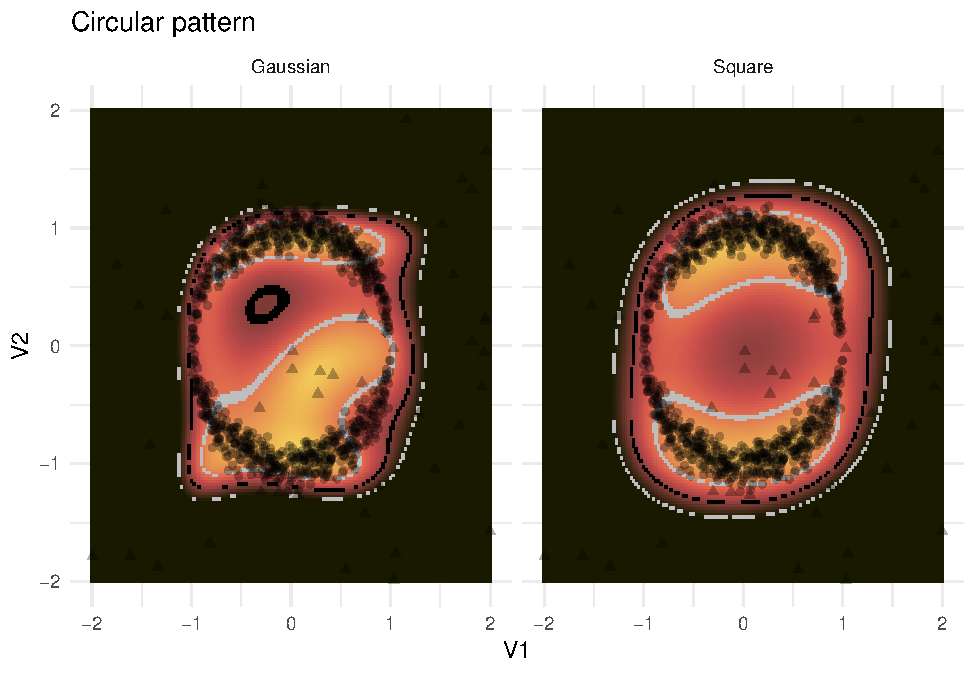
\includegraphics[width=1\linewidth]{outlier-detection_files/figure-latex/kpca-circ-1} 

}

\caption{Example application of the kernel PCA to the circular pattern}\label{fig:kpca-circ}
\end{figure}

Even though some inliers might be classified as outliers according to
the threshold of 2 standard deviations, any other threshold recognizes
the inliers. The Gaussian kernel even recognizes that the points within
the circle should be classified as outliers, as well. On the whole, both
methods results correspond to our intuition and are fairly strict.

In contrast, the Gaussian kernel is too strict with respect to the
quadratic pattern in \ref{fig:kpca-quad}.

\begin{figure}

{\centering 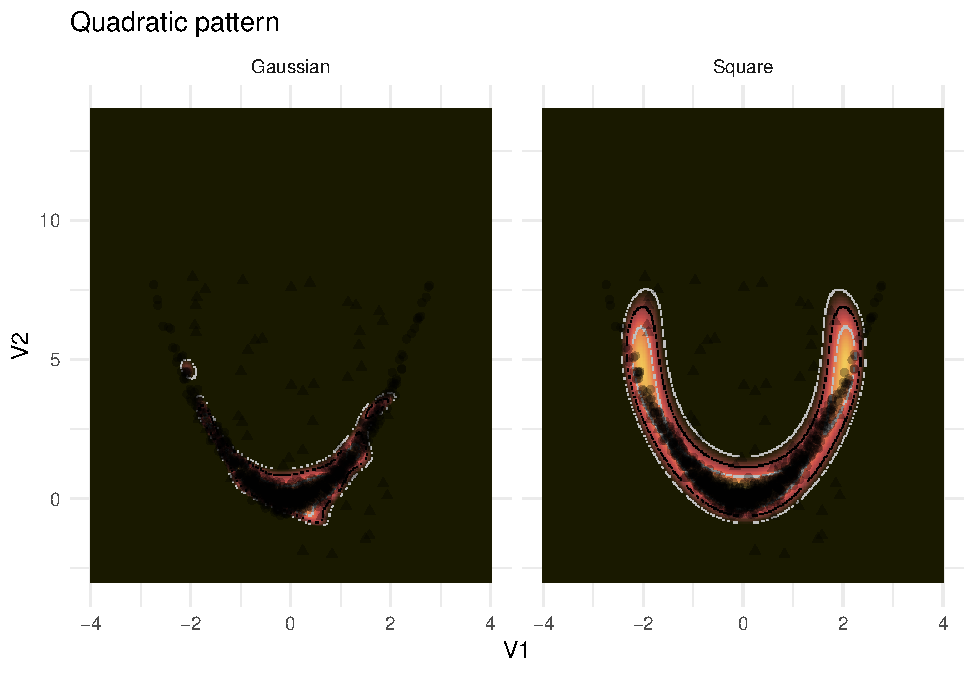
\includegraphics[width=1\linewidth]{outlier-detection_files/figure-latex/kpca-quad-1} 

}

\caption{Example application of the kernel PCA to the quadratic pattern}\label{fig:kpca-quad}
\end{figure}

However, the polynomial kernel captures the pattern almost perfectly.

Finally, both methods struggle with the sinusoidal pattern in
\ref{fig:kpca-trig}. The polynomial seems insufficiently complex for
this pattern whereas the more local Gaussian kernel does not recognize
the overall pattern but only some denser points. The latter is, on the
whole, too restrictive, however.

\begin{figure}

{\centering \includegraphics[width=1\linewidth]{outlier-detection_files/figure-latex/kpca-trig-1} 

}

\caption{Example application of the kernel PCA to the sinusoidal pattern}\label{fig:kpca-trig}
\end{figure}

These examples demonstrate that kernel PCAs can yield powerful results
but still need to be assessed carefully. Fitting the hyperparameters and
using certain evaluation criteria can help ensure a good result. In
particular the quadratic kernel seems to be adept at handling nonlinear
patterns which are not too complex.

\hypertarget{discussion-2}{%
\subsection{Discussion}\label{discussion-2}}

In summary, the great flexibility is the decisive advantage of kernel
PCA. This method, together with the right kernel, can recognize and
handle arbitrary data. Such flexibility, however, has a downside, as
well. Due to the many hyperparameters, the method is susceptible to
overfitting. Moreover, it is more difficult to fit such a model compared
to a linear model which is relatively easy to understand and apply.

Another advantage which comes with the kernel trick is that any
similarity measure can be used for kernel PCA as long as it yields a
positive semi-definite matrix. This means that kernel PCA can be applied
to topics as diverse as graph analysis, spatiotemporal analysis and text
analysis.

\hypertarget{neural-networks}{%
\section{Neural networks}\label{neural-networks}}

I will conclude with a short excursion to outlier detection using
\emph{neural networks}.

\emph{Neural networks} are a Machine Learning algorithm which is adept
at approximating complex, non-linear patterns. Their application to
outlier detection can well be motivated by considerations in the field
of data compression. We compress data by identifying its decisive
properties and attempting to summarize it by as few numbers as possible.
For instance our perception summarizes any colour by three numbers: its
redness, blueness and greenness. Three numbers are therefore sufficient
to describe our perception of any colour. These summaries are often
nonlinear which is why neural networks are suitable for handling them.
Broadly speaking, neural networks consist of several layers of nodes
where a weighted sum of all the nodes in one layer feeds into the node
of the next layer. Any layer therefore only depends on the values in the
layer before \footnote{Neural networks can also encompass more general
  structures but the one described here is the most suitable for outlier
  detection.}.

The idea of outlier detection using neural networks is therefore the
following: we map the input layer (i. e. all variables) through several
intermediate layers to the mid-layer which contains of a lower number of
nodes. Then we reflect this architecture and finally attempt to predict
the same variables from the initial variables by following the
\emph{backpropagation algorithm}. The better we perform at predicting
the input from the input the better our compression using the mid-layer
works. On the other hand, those observations which cannot be predicted
very well apparently do not adhere to the general pattern.

In R, neural networks can, for instance, be fitted using the package
\texttt{keras}. \citep{keras} Due to the many hyperparameters such as
number of layers and number of nodes in each layer, fitting a neural
network is a complex undertaking which goes beyond the scope of this
report. An introduction to fitting neural networks can be found in
section 10.7 of \citet{Aggarwal2015}.

I will conclude this report by revisiting the introduction in which we
discussed outlier detection using predictive coding in the brain.
Interestingly, a recent paper by \citet{Whittington2017} demonstrated
equivalency of neural networks and predictive coding under certain
conditions. This has two implications: on the one hand, neural networks
might bring us closer to understanding how our brain detects outliers.
This is more important in outlier detection than in other statistical
fields as outlier detection is more vaguely defined and depends more
strongly on human intuition. On the other hand, predictive coding might
contain new suggestions for complex probablistic outlier detection
methods.

\hypertarget{summary}{%
\chapter{Summary}\label{summary}}

In this report, I have introduced the field of outlier detection using
regression by looking at prominent and useful linear methods before
extending these to their non-linear version. I have provided
applications of these methods within R and looked at example
applications to artifically created datasets. To assess these
application, I have developed the \emph{Z plot} which uses a simple
heuristic to compare different outlier scores without preparation.

\bibliography{outlier-detection.bib}


\end{document}
